              
% --------------------------------------------------------------
% This is all preamble stuff that you don't have to worry about.
% Head down to where it says "Start here"
% --------------------------------------------------------------
 
\documentclass[11pt]{article}
\usepackage[utf8]{inputenc} 
\usepackage[margin=1in]{geometry}
\usepackage{graphicx}
\usepackage{float}
\usepackage{hyperref} 
\usepackage{amsmath,amsthm,amssymb}
\usepackage[table]{xcolor}
 
\newcommand{\N}{\mathbb{N}}
\newcommand{\Z}{\mathbb{Z}}
 
\newenvironment{theorem}[2][Theorem]{\begin{trivlist}
\item[\hskip \labelsep {\bfseries #1}\hskip \labelsep {\bfseries #2.}]}{\end{trivlist}}
\newenvironment{lemma}[2][Lemma]{\begin{trivlist}
\item[\hskip \labelsep {\bfseries #1}\hskip \labelsep {\bfseries #2.}]}{\end{trivlist}}
\newenvironment{exercise}[2][Exercise]{\begin{trivlist}
\item[\hskip \labelsep {\bfseries #1}\hskip \labelsep {\bfseries #2.}]}{\end{trivlist}}
\newenvironment{reflection}[2][Reflection]{\begin{trivlist}
\item[\hskip \labelsep {\bfseries #1}\hskip \labelsep {\bfseries #2.}]}{\end{trivlist}}
\newenvironment{proposition}[2][Proposition]{\begin{trivlist}
\item[\hskip \labelsep {\bfseries #1}\hskip \labelsep {\bfseries #2.}]}{\end{trivlist}}
\newenvironment{corollary}[2][Corollary]{\begin{trivlist}
\item[\hskip \labelsep {\bfseries #1}\hskip \labelsep {\bfseries #2.}]}{\end{trivlist}}
 
\begin{document}
 
% --------------------------------------------------------------
%                         Start here
% --------------------------------------------------------------
 
\setlength\parindent{0pt}
%\renewcommand{\qedsymbol}{\filledbox}
 
\title{Assignment 1: Game theory}%replace X with the appropriate number
\author{Pierre Gérard (ULB)\\ %replace with your name
INFO-F-409 - Learning dynamics} %if necessary, replace with your course title
 
\maketitle

\begin{exercise}{1} The Hawk-Dove game
\end{exercise}

\begin{figure}[H]
   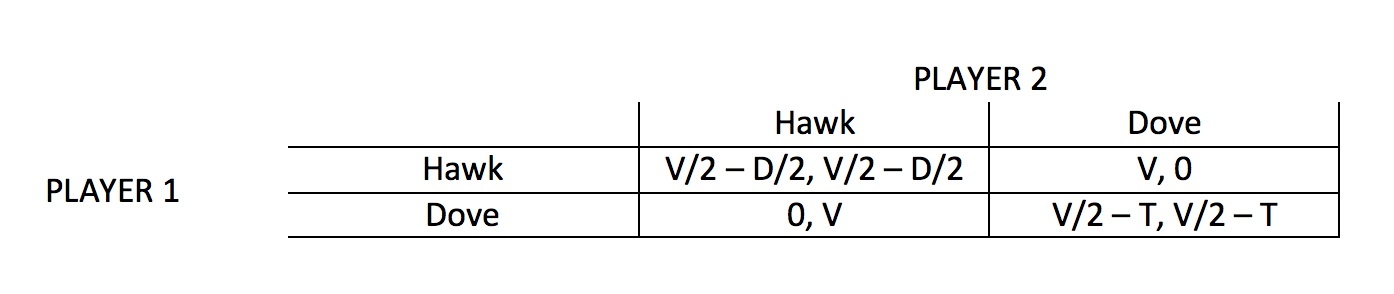
\includegraphics[width=\textwidth]{img/exo1.png}
\end{figure}


\paragraph{Mixed strategy Nash Equilibria}

.

To have mixed strategy, we have to assume that $\frac{V}{2}-\frac{D}{2}<0$ and that $\frac{V}{2}-T<0$. \\

There are two obvious Pure Strategy Nash Equilibrium which are (Dove,Hawk) and (Hawk,Dove). \\

Let's start by calculating the mixed strategy for Player 1. We know that the probability of scenario in which Player 1 win V is $0.5$ and the probability of losing is also $0.5$.\\

Let's define $p$ as the probability that Player 1 play Hawk.\\

So the Bernouilli payoff function is for the utility of the second player :\\

$U_2 (Hawk) = p (\frac{V}{2}-\frac{D}{2}) + (1-p) V$ 

\vspace{2mm}
$U_2 (Dove) = p * 0 + (1-p)(\frac{V}{2}-T)$.\\

To solve the mixed strategy, let's resolve the following equation : \\

$U_2 (Hawk) = U_2 (Dove)$

\vspace{2mm}
$p (\frac{V}{2}-\frac{D}{2}) + (1-p) V = p * 0 + (1-p)(\frac{V}{2}-T)$

\vspace{2mm}
$ p = \frac{V+2T}{D+2T}$ \\

So, both player play Hawk with probability of $ p = \frac{V+2T}{D+2T}$ and Dove with complementary probability. \\

Note that if the hypothesis above are not respected for V,D,T, we won't have a MSNE but only PSNE. For example if $V/2-D/2>0$, then players play (Hawk,Hawk) is equilibrium.

\paragraph{Displaying} 

.

Displaying become more beneficial than escalating when :

\vspace{2mm}
$U_2 (Dove) > U_2 (Hawk)$

\vspace{2mm}
$p * 0 + (1-p)(\frac{V}{2}-T) > p (\frac{V}{2}-\frac{D}{2}) + (1-p) $

\vspace{2mm}
$p > \frac{V+2T}{D+2T} $



\begin{exercise}{2} Which social dilemma?
\end{exercise}

For player A, each social dilemma has an equal probability of $\frac{1}{3}$ of being played. Player A does not know and which game will be play and has to choose a strategy in the set $\{C, D \}$. \\

On the other hand, Player B knows in advance in which game he will be playing and had to choose a strategy in $\{C, D \}$ for every game, resulting in a strategy in the set $\{ CCC, CDC, CCD, ... \}$. \\

Let's modelize this uncertain environment to find the best strategy for each player in response to the other player.

\paragraph{Player A}

To find the best response of player A for a choice of player B, let's find the payoff of player A for every strategy of Player B. \\

$(C - CCC): \frac{1}{3}*2 + \frac{1}{3}*5 + \frac{1}{3}*2 = 3 $ \\

$(D - CCC): \frac{1}{3}*5 + \frac{1}{3}*2 + \frac{1}{3}*5 = 4 $ \\

$(C - DCC): \frac{1}{3}*0 + \frac{1}{3}*5 + \frac{1}{3}*2 = \frac{7}{3} $ \\

$ ... $ \\

When apply to every combination of strategy, this give us the following table.

\begin{figure}[H]
   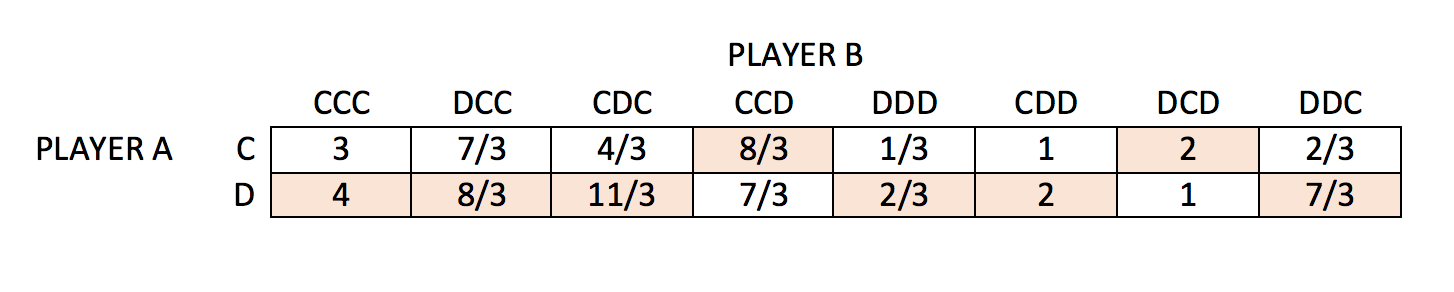
\includegraphics[width=\textwidth]{img/exo2-table1.png}
\end{figure}

Like in the slides, red means best strategy. So here, for example if Player B choose $CCC$, the best response for Player A would be to play $D$.


\paragraph{Player B}

To find the best response of player B to a strategy of player A, let's find the payoff of player B for every strategy of Player A.

\begin{figure}[H]
   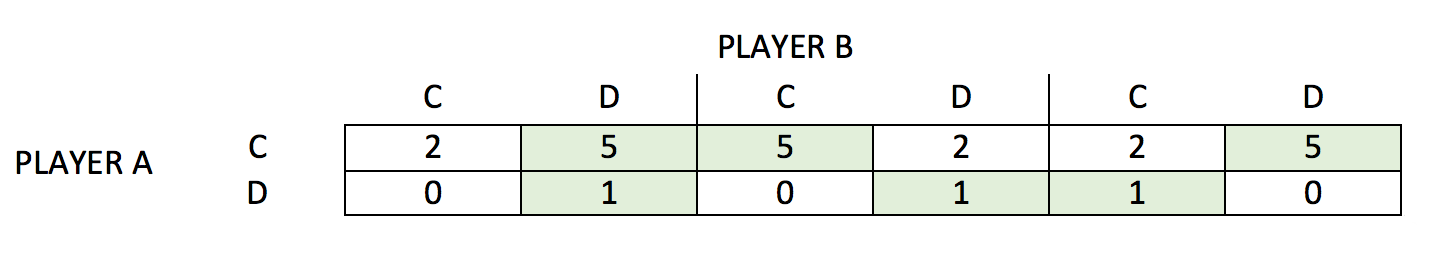
\includegraphics[width=\textwidth]{img/exo2-table2.png}
\end{figure}

The response that will be best for Player B if A choose $C$ is ${CCD}$ and $DDC$ if player A choose $D$. \\

\textbf{When matching the colour in the two tables above we can find two NE :
$(C - DCD)$ and $(D - DDC)$ }

\begin{exercise}{3} Sequential truel
\end{exercise}

 
\begin{figure}[H]
   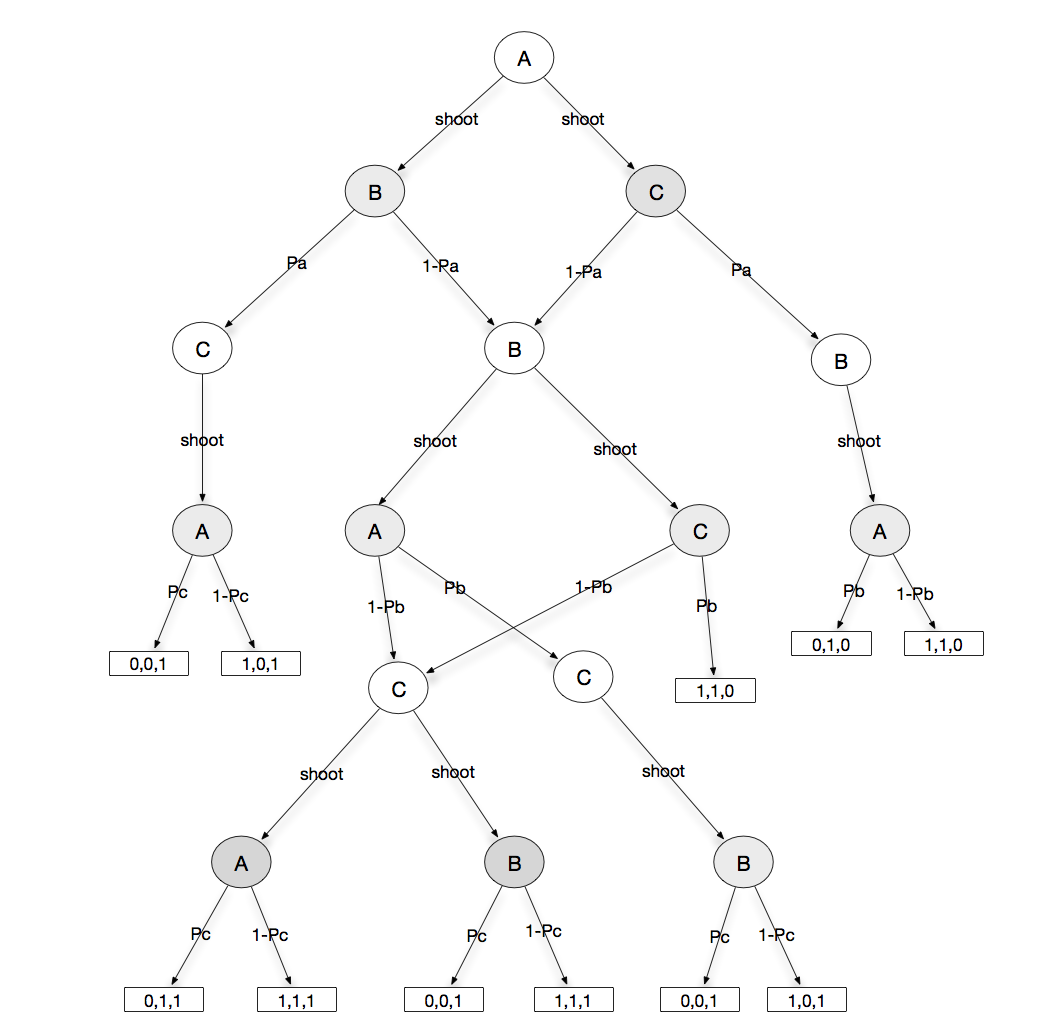
\includegraphics[width=\textwidth]{img/exo3.png}
\end{figure}

In the drawing above, we suppose that a survival give a reward of 1 and death give zero. So, for example, a result 0,0,1 means that only Player C survive. \\

It is best for Player A 's chance of survival to shoot someone, because then if he succeed only one player will be able to fire a shot a him. The best target for him would obviously be to shot the best shooter.

\begin{itemize}
	\item If he chooses $B$, the expected payoff would be $Pa (1-Pc)$
	\item If he chooses $C$, the expected payoff would be $Pa (1-Pb)$
\end{itemize}

Player will choose the one giving him the best payoff. Knowing that, we can say that it is better for B to have Pb smaller than Pc because Player A would rationally choose to shot C and he would increase his chance or survival. The same reasoning can be make for Player C, we can say that it is better for C to have Pc smaller than Pb because Player A would rationally choose to shot B and he would increase his chance or survival. So being a bad shooter \textit{(weakness)} increase a player chance of survival \textit{(is strength)}.

It is not possible to find the sub-game perfect equilibria of the game without knowing the order of $Pa, Pb, Pc$, in other words without knowing which one is bigger than other one. But as said above, Player A will shoot at Player B or Player C depending on which one has the biggest probability. If Player A misses or choose C, Player B will rationally always target Player C because Player A is not a thread anymore. And if at the end Player C is still alive, he does not have any preferences.

 

\end{document}







































              